\documentclass[man]{apa7}
\usepackage[american]{babel}
\setcounter{tocdepth}{4}
\setcounter{secnumdepth}{4}
\usepackage{csquotes}
\usepackage{titlepic}
\usepackage{graphicx}
\usepackage{adjustbox}

\usepackage{amsfonts}

\usepackage[style=apa,backend=biber]{biblatex}
\usepackage{lipsum}
\DeclareLanguageMapping{american}{american-apa}
\addbibresource{mybibfile.bib}
\usepackage{fancyhdr}
\pagestyle{fancy}
\fancyhf{}
\lhead{\textit{Graduation Project}}
\rhead{\thepage}


\begin{document}
\begin{titlepage}
\centering
{\large \textbf{ Istanbul Technical University - Science and Letters Faculty}}\\
{\large \textbf{Mathematics Engineering Program}}\\[4\baselineskip]

\includegraphics[scale = 1.5]{itülogo.png}\\[6\baselineskip]
{\LARGE \textbf{Graduation Project}}\\[2\baselineskip]

{\Large Student Name: Arif Çakır}\\
{\large Student Number: 090190355}\\
{\large Course: MAT4091E}\\
{\large Advisor: Prof. Dr. Atabey Kaygun}\\
{\large Submission Date: \today}\\
\end{titlepage}
\tableofcontents
\pagebreak

\section{Introduction}
Language is a fundamental aspect of human communication and one of the most common ways to pass on information and culture throughout history. Due to its nature of encapsulating information, language is studied by linguists throughout the years. Thanks to this scientific foundation, machine learning, and computer science are also advanced upon this topic. Natural Language Processing (NLP) is the subfield of machine learning that studies the processing of human language by computers. One of the most popular NLP techniques in recent years is Word Embedding, which represents words as vectors in semantic space that allows applying mathematical operations on them to analyse. Word Embedding can be used on various subjects such as text classification, translation, and sentiment analysis with promising results. It is aimed in this paper to study several Word Embedding techniques and their applications. The aim is to create a model by applying various Word Embedding models and with the help of this model, describing the relationships and similarities of languages.

The rest of the paper is organised as follows: In Section 2, information about Word Embedding in general and several Word Embedding techniques are provided. Word Embedding techniques touched on in the paper are Term Frequency (TF), Inverse Document Frequency (IDF), Word2Vec, Global Vectors for Word Representation (GloVe), Bidirectional Encoder Representations from Transformers (BERT). This is followed by Section 3 which introduces the dataset Divine Comedy by Dante Aligheri. After that, several Word Embedding models are applied to the dataset in Section 4, and the outputs of those models are analysed in Section 5. Finally paper ends with some discussion and a conclusion in Section 6.

\section{Word Embedding Techniques}
Word Embedding is one of the most popular natural language processing techniques due to its vector representation of the words. As Agarwal stated, capturing semantic meaning of the words in a vector of text is the ambition of the word embedding techniques \cite(Agarwal, 2022). With respect to that, some of the most popular word embedding techniques will be studied in this section. Those techniques are TF, which counts rarity of words; IDF, which counts rarity of words; Word2Vec, which uses cosine similarity; GloVe, which captures co-occurrence of words; and BERT, family of masked-language models introduced by Google.

\subsection{Term Frequency - Inverse Document Frequency}
Term Frequency (TF) is a word embedding technique which counts the occurrence of the words in a document. TF can be shown as

\begin{equation}
TF(i) =   \frac{\log(Frequency(i,j))}{\log(TotalNumber(j))}.
\end{equation}

where $Frequency(i,j)$ is the frequency of a word that occurred in a j word document and $TotalNumber(j)$ is the total number of the words in the document.

On the other hand, Inverse Document Frequency (IDF) is practically the opposite of the TF method. In this method, algorithm relies on the information that gained from the words which are rarely used. IDF can be written as

\begin{equation}
IDF (i) = \log (\frac{TotalNumber(j)}{Frequency(j,i)}).
\end{equation}

where $Frequency(i,j)$ is the frequency of a word that occurred in a j word document and $TotalNumber(j)$ is the total number of the words in the document.

TF-IDF mainly shows the degree of relevancy of word i in the document j, while the main disadvantage of TF-IDF is it does not grasp contextual relationship between the words. As Kınık and Güran stated, TF-IDF does not capture semantic relationship between words, and accepts them as independent values \cite(Kınık and Güran,2021). Due to TF-IDF's lack of capturing semantic relationship of the words, TF-IDF mainly used to detect stop words.

\subsection{Word2Vec}
Word2Vec is a word embedding model that was published by researchers led by Tomáš Mikolov at Google in 2013. As stated in Gensim documentations (n.d.), words are embeded in lower-dimensional vector space by Work2Vec. In this vector space, vectors which have similarity of context between them are close to each other while words that have different meanings are distant to each other. After that, Word2Vec uses cosine similarity metric to measure similarity of the words. If cosine value of two words is 0, then words do not hold similarity. If cosine value of two words  is 1, then the words are overlapping. Due to that, Word2Vec model is mostly used in semantic analysis. On the other hand, the main disadvantage of Word2Vec model is that it can not handle out of vocabulary words well. The words not presenting in training data is called out of vocabulary words. As Chandran stated (2020), a random vector representation is assigned for out of vocabulary words by Word2Vec, and they can be not optimal. There are two neural network based variations of Word2Vec: Skip-Gram and Continuous Bag of Words.

\subsubsection{Skip-Gram Algorithm}
One of the Word2Vec model architectures is Skip-Gram Algorithm. Dive Into Deep Learning (n.d) states that a word can be used for generating its surrounding words in skip-gram model. For example, if the sentence "the man loves his son" is taken and "loves" is chosen as the center word, then skip-gram model considers the conditional probability for generating the words. Due to this approach, each word has a two dimensional vector representations in skip-gram model. 

\begin{center}

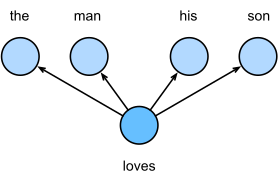
\includegraphics[scale=1]{skip-gram.png}

\textbf{Figure 1:} Skip-Gram model architecture, from Dive Into Deep Learning\\[2\baselineskip]

\end{center}

According to Dive Into Deep Learning, for any word with index $\mathit{i}$ in the directory, $\mathbf{v_\mathit{i}} \in \mathbb{R}^d$ and $\mathbf{u_\mathit{i}} \in \mathbb{R}^d$ are its two vector representations, where $\mathbf{v_\mathit{i}}$ is when the word is used as the "center word" and $\mathbf{u_\mathit{i}}$ is when the word is used as the "context word". If $\mathit{w_o}$ is any context word and $\mathit{w_c}$ is given center word, then conditional probability of generating $\mathit{w_o}$ can be modelled as

\begin{equation}
P(w_o | w_c) = \frac{exp(\mathbf{u_\mathit{o}}^\top \mathbf{v_\mathit{c}})}{\sum_{i \in \mathcal{V}} exp(\mathbf{u_\mathit{i}}^\top \mathbf{v_\mathit{c}})}.
\end{equation}

where $ \mathcal{V}$ is the vocabulary index set. If a text sequence of length $T$ is given and word at time step $t$ is denoted as $\mathit{w}^t$, then likelihood function of skip-gram model for context widow size $m$ is as following:

\begin{equation}
\prod_{t=1}^T \prod_{-m \le j \le m , j \neq 0} P(w^{t+j} | w^t).
\end{equation}

The skip-gram model parameters are center word and context word vector for each word in the corpus. In order to train skip-gram model, given loss function must be minimized:

$$ -\sum_{t=1}^T \sum_{-m \le j \le m, j \neq 0} logP(w^{(t+j)} | w^{(t)}).$$

Moreover, while using (stochastic) gradient descent to minimize the loss function, gradients of log conditional probability must be obtained. For center word $w_c$ and context word $w_o$, log conditional probability is

\begin{equation}
logP(w_o|w_c) = \mathbf{u}_o^\top \mathbf{v}_c - log(\sum_{i \in \mathcal{V}} exp(\mathbf{u}_i^\top \mathbf{v}_c)).
\end{equation}

And the gradient of center word $\mathbf{v}_c$ can be obtained as

\begin{equation}
\frac{\partial P(w_o | w_c)}{\partial \mathbf{v}_c} = \mathbf{u}_o - \sum_{j \in \mathcal{V}} P(w_o|w_c)\mathbf{u}_j.
\end{equation}

After this calculations, Dive Into Deep Learning states that we obtain center word vector $\mathbf{v}_i$ and context word vector $\mathbf{u}_i$ for index $i$ in the dictionary.

\subsubsection{Continuous Bag of Words}
The other variant of Word2Vec model is continuous bag of words (CBOW). The main difference between skip-gram and CBOW is instead of generating surrounding words respect to center word, CBOW generates center word with the help of surrounding words. If the same example "the man loves his son" is taken for CBOW model, instead of generating surrounding words based on center word "loves", the model generates center word "loves" from its surroundings.
\\[2\baselineskip]

\begin{center}
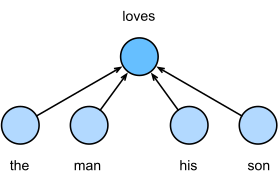
\includegraphics[scale=1]{cbow.png}

\textbf{Figure 2:} CBOW model architecture, from Dive Into Deep Learning\\[2\baselineskip]

\end{center}

According to Dive Into Deep Learning (n.d.), in order to calculate conditional probability, context word vectors are averaged because there are multiple words. For any word with index $i$ in the dictionary, $\mathbf{v_\mathit{i}} \in \mathbb{R}^d$ is the context word while $\mathbf{u_\mathit{i}} \in \mathbb{R}^d$  is the center word. It can be seen that meanings are switched compared to skip-gram model. While $w_o,...,w_{o_{2m}}$ the conditional probability of generating center word $w_c$ can be modelled as following:

\begin{equation}
P(w_c|w_o,...,w_{o_{2m}}) = \frac{exp(\frac{1}{2m}u_c^\top(\mathbf{v}_{o_1}+...+\mathbf{v}_{o_{2m}}))}{\sum_{i \in \mathcal{V}} exp(\frac{1}{2m}u_c^\top(\mathbf{v}_{o_1}+...+\mathbf{v}_{o_{2m}}))}.
\end{equation}

For simplicity, $\mathcal{W}_o = \{ w_o,...,w_{o_{2m}}\}$ and $\bar{\mathbf{v}}_o = (\mathbf{v}_{o_1}+...+\mathbf{v}_{o_{2m}})/(2m)$. Then equation given above is simplified as following:

\begin{equation}
P(w_c | \mathcal{W}_o) = \frac{exp(u_c^\top \bar{\mathbf{v}}_o)}{\sum_{i \in \mathcal{V}} exp(u_i^\top \bar{\mathbf{v}}_o)}.
\end{equation}

Furthermore, Dive Into Deep Learning (n.d.) states that if the length of a text sequence is $\mathit{T}$ and the word at time $t$ is $w^{(t)}$, then for context window of size $m$ the likelihood function of CBOW model is

\begin{equation}
\prod_{t=1}^T P(w^{(t)}| w^{(t-m)},..., w^{(t-1)},w^{(t+1)},...,w^{(t+m)}).
\end{equation}

Due to CBOW and skip-gram models being similar, training them also almost same. According to Dive Into Deep Learning, to train CBOW model, maximum likelihood estimation of CBOW model is equal to minimization of following loss function

\begin{equation}
- \sum_{t=1}^T logP(w^{(t)} | w^{t-m)} ,..., w^{(t-1)} ,w^{(t+1)}, ...,w^{(t+m)}).
\end{equation}

where

\begin{equation}
logP(w_c | \mathcal{W}_o) = \mathbf{u}_c^\top \bar{\mathbf{v}}_o - log(\sum_{i \in \mathcal{V}} exp(\mathbf{u}_i^\top \bar{\mathbf{v}}_o)).
\end{equation}

Through differentiation, gradient with respect to any cotext word vector $\mathbf{v}_{o_i}$ can be obtained as

\begin{equation}
\frac{\partial log P(w_c| \mathcal{W}_o )}{\partial \mathbf{v}_{o_i}} = \frac{1}{2m}(\mathbf{u}_c - \sum_{j \in \mathcal{V}} P(w_j| \mathcal{W}_o \mathbf{u}_j)).
\end{equation}

Furthermore, gradients of other vectors can be obtained with the same way.

\subsection{Global Vectors for Word Representation}
Global Vectors for Word Representation (GloVe) is an unsupervised learning algorithm that developed by scientist led by Jeffery Pennington in Stanford University. Unlike Word2Vec, GloVe captures global contextual information of words by calculating a global word-word co-occurrence matrix. For example, in a large corpus, the word "liquid" more likely to co-occur with "water" than "ice", but word "solid" more likely to co-occur with "ice" than "steam". According to Agarwal, only local context of words is captured by Word2Vec (Agarwal, 2022). On the other hand, entire corpus is considered by GloVe and a large matrix that can capture co-occurrence of words within the corpus is created.
\\[2\baselineskip]

\begin{center}
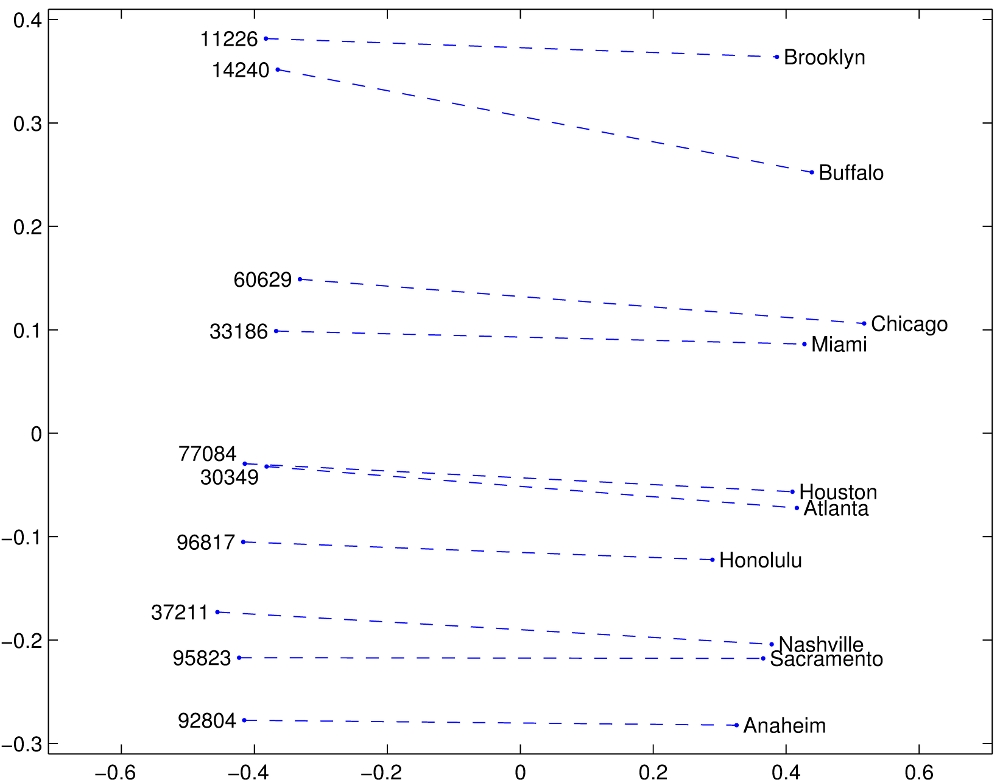
\includegraphics[scale=3]{city_zip.jpg}

\textbf{Figure 3:} GloVe vectors capturing relation between city and zip code, from Stanford University\\[2\baselineskip]

\end{center}

Agarwal continues by GloVe has the combination of the advantages of two-word vector learning methods: matrix factorization like latent semantic analysis (LSA) and local context window method (like Skip-Gram or CBOW). LSA is the technique that analyses the relationship between a set of documents and the terms they contain by using singular value decomposition. 

Furthermore, the GloVe method's computational time is reduced by a rather simpler least square error function. As it is stated in Dive Into Deep Learning, Glove makes three changes to skip-gram model square loss (n.d.). where vectors $\mathbf{v_\mathit{i}} \in \mathbb{R}^d$ and $\mathbf{u_\mathit{i}} \in \mathbb{R}^d$ keep same representations as skip-gram model, those there changes are as following:

1. Using variables $p'_{ij} = x_{ij}$ and $q'_{ij} = exp(\mathbf{u}_j^\top \mathbf{v}_i)$ that are not probabilistic distributions. After taking their logarithms, the squared loss term becomes $(log(p'_{ij})-log(q'_{ij}))^2 = (\mathbf{u}_j^\top \mathbf{v}_i - log (x_{ij}))^2$.

2. For each word $w_i$, adding two scalar model parameters: the center word bias $b_i$ and context word bias $c_i$.

3. Replacing the weight of each loss term $h(x_{ij}$ where $h(x)$ is increasing in the interval of $[0,1]$.
 
Therefore, loss function of GloVe is:
\begin{equation}
\sum_{i \in \mathcal{V}} \sum_{j \in \mathcal{V}} h(x_{ij})(u_j^\top \mathbf{v}_i + b_i +c_j -log(x_{ij}))^2
\end{equation}


Where suggested choice for $h(x)$ is if $x < c$ , then $h(x) = (x/c)^\alpha$, else $h(x) = 1$. 

Finally, when compared to Word2Vec GloVe handles out of vocabulary words better. Due to that, GloVe performs better in word analogy and named entity recognition tasks. 

\subsection{Bidirectional Encoder Representations from Transformers}
Created by researchers at Google in 2018, Bidirectional Encoder Representations from Transformers (BERT) is a family of masked-language models. Before discussing BERT; terms context-independent, context-sensitive, task-specific and task-agnostic must be discussed.

A context-independent function $f(x)$ only takes token $x$ as its input. Due to the complex semantics and synonyms in natural languages, context-independent representations miss the meaning of the words in some cases. For example, the word "bank" can be used in both the sentence "I sat by the bank and enjoyed the view of the river." and the sentence I went to the bank to deposit some money". A context-independent algorithm might miss the difference between this cases.

On the other hand, context-sensitive function $f(x,c(x))$ is dependent to both token $x$ and context $c(x)$. According to Dive Into Deep Learning, some of the most popular context sensitive representations are language-model-augmented sequence tagger (TagLM), Context Vectors (CoVe), and ELMo (Embeddings from Language Models).

When it comes to task-specific and task-agnostic representation, task-specific representation is when a model is optimized to a specific task, while a task-agnostic representation is when model is independent from a task based architecture. For instance, ELMo is an task-specific solution while it is not necessary to create specific architecture for each NLP task. The Generative Pre-Training  (GPT) model is a context-sensitive, task-agnostic representation. However, according to Dive Into Deep Learning, GPT only look left to right because of autoregressive nature of natural languages. For example, the sentences "A crane is flying." and "A crane is crashed." is taken, because of word "crane" being sensitive to context in its left, GPT will return the same representation of "crane".

\section{Dataset}

\subsection{Information About the Dataset}

\subsection{Preparation of the Dataset}

\section{Applying Models to the Dataset}

\subsection{Skip-Gram Algorithm}

\subsection{Continuous Bag of Words}

\section{Analysis and Visualization}

\section{Discussion}

\end{document}